  
\chapter{Related Work}
\label{chap:related_work}

\section{Natural Language Processing}
\label{sec:rel_nlp}

\section{Language Models}
\label{sec:relwork-language-models}

A statistical language model assigns assigns a probability to a sequence of m
words $P(w_1,\ldots,w_m)$ by means of a probability distribution. 
This probability can be obtained from the probability of
each word given the context of words preceding it using the chain rule of probability \cite{Bengio:2008}:

\begin{equation}
\label{eq:lm_probability}
 P(w_1, w_2, \ldots, w_{t-1},w_t) = P(w_1) P(w_2|w_1) P(w_3|w_1,w_2) \ldots 
  P(w_t | w_1, w_2, \ldots w_{t-1}).
\end{equation}

Most probabilistic language models  approximate $P(w_t | w_1, w_2, \ldots
w_{t-1})$ using a fixed context of size $n-1$, i.e. using  $P(w_t | w_{t-n+1}, \ldots w_{t-1})\ ,$.



\section{N-Grams based language models}
\label{sec:n-gram-lm}

\section{Neural Network Language Models}
\label{sec:nnlms-intro}

As its name describes, is a language model based on a \ac{NN}, exploiting their
ability to learn distributed representations to reduce the impact of the
curse of dimensionality \cite{Bengio:2008}. In other words, a \ac{NN} is
used to estimate the probability described  by equation (\ref{eq:lm_probability}) based on a sequence of
previous words.

The advantage  using  distributed representations  is that they allows
the model to generalize well to sequences that are not in the set of training
word sequences, but that are similar in terms of their features. Because neural networks tend to map nearby inputs
to nearby outputs, the predictions corresponding to word sequences with
similar features are mapped to similar predictions. \cite{Bengio:2008,Bengio:2003:NPL:944919.944966}

However, Due to the nature the architecture, many of these models suffer
performance issues the hidden layers and output layer of the \ac{NN} are
generally the bottleneck.  In order to be able to compare the different
models in term of their complexity it is necessary then to define the
complexity of  their architecture. All of these models have a complexity proportional to 
\cite{DBLP:journals/corr/abs-1301-3781}:

\begin{center}
\begin{equation} O = E \times T \times Q,   \end{equation}
\end{center}

where $E$ is number of the training epochs, $T$ is the number of the words in
the training set and $Q$ depends on each architecture. Common choice is $E$ = 3-50 and $T$ up to one billion.
All models are trained using stochastic gradient descent and backpropagation
\cite{Bengio:2003:NPL:944919.944966}\cite{DBLP:journals/corr/abs-1301-3781}.

The following subsection describe each of the most popular  model and their
associated complexity $Q$.

\subsection{Feedforward Neural Network Language Model}
\label{subsec:fwd-neural-net-lm}

% Section \ref{sec:relwork-language-models} described the generalities of
% language models in the context of \ac{NLP}.  In that section we described
% that the 

In the \ac{FNNLM} that was introduced by Bengio
\cite{Bengio:2003:NPL:944919.944966},  the probabilistic prediction $P(w_t | w_{t-n+1}, \ldots w_{t-1})$ described
in equation (\ref{eq:lm_probability}) is obtained as follows. First, each word $w_{t-i}$ (represented
with an integer in $[1,N]$) in the  $n-1$-word context is mapped
to an associated $d$-dimensional feature vector $C_{w_{t-i}}\ ,$ which is
column $w_{t-i}$ of parameter matrix $C\ .$ Vector $C_k$
contains the learned features for word $k\ .$
Let vector $x$ denote the concatenation of these $n-1$
feature vectors:
\begin{equation}
  x = (C_{w_{t-n+1},1}, \ldots, C_{w_{t-n+1},d}, C_{w_{t-n+2},1}, \ldots C_{w_{t-2},d}, C_{w_{t-1},1}, \ldots C_{w_{t-1},d}).
\end{equation}
The probabilistic prediction of the next word, starting from $x$
is then obtained using a standard artificial neural network architecture
for probabilistic classification, using the softmax activation function at the output units (Bishop, 1995):
\begin{equation}
 P(w_t=k | w_{t-n+1}, \ldots w_{t-1}) = \frac{e^{a_k}}{\sum_{l=1}^N e^{a_l}}
\end{equation}
where
\begin{equation}
 a_k = b_k + \sum_{i=1}^h W_{ki} \tanh(c_i + \sum_{j=1}^{(n-1)d} V_{ij} x_j)
\end{equation}
where the vectors $b,c$ and matrices $W,V$ are also
parameters (in addition to matrix $C$). Let us denote
$\theta$ for the concatenation of all the parameters.
The capacity of the model is controlled by the number of hidden units $h$
and by the number of learned word features $d\ .$ 


\begin{figure}[h]
    \centering
    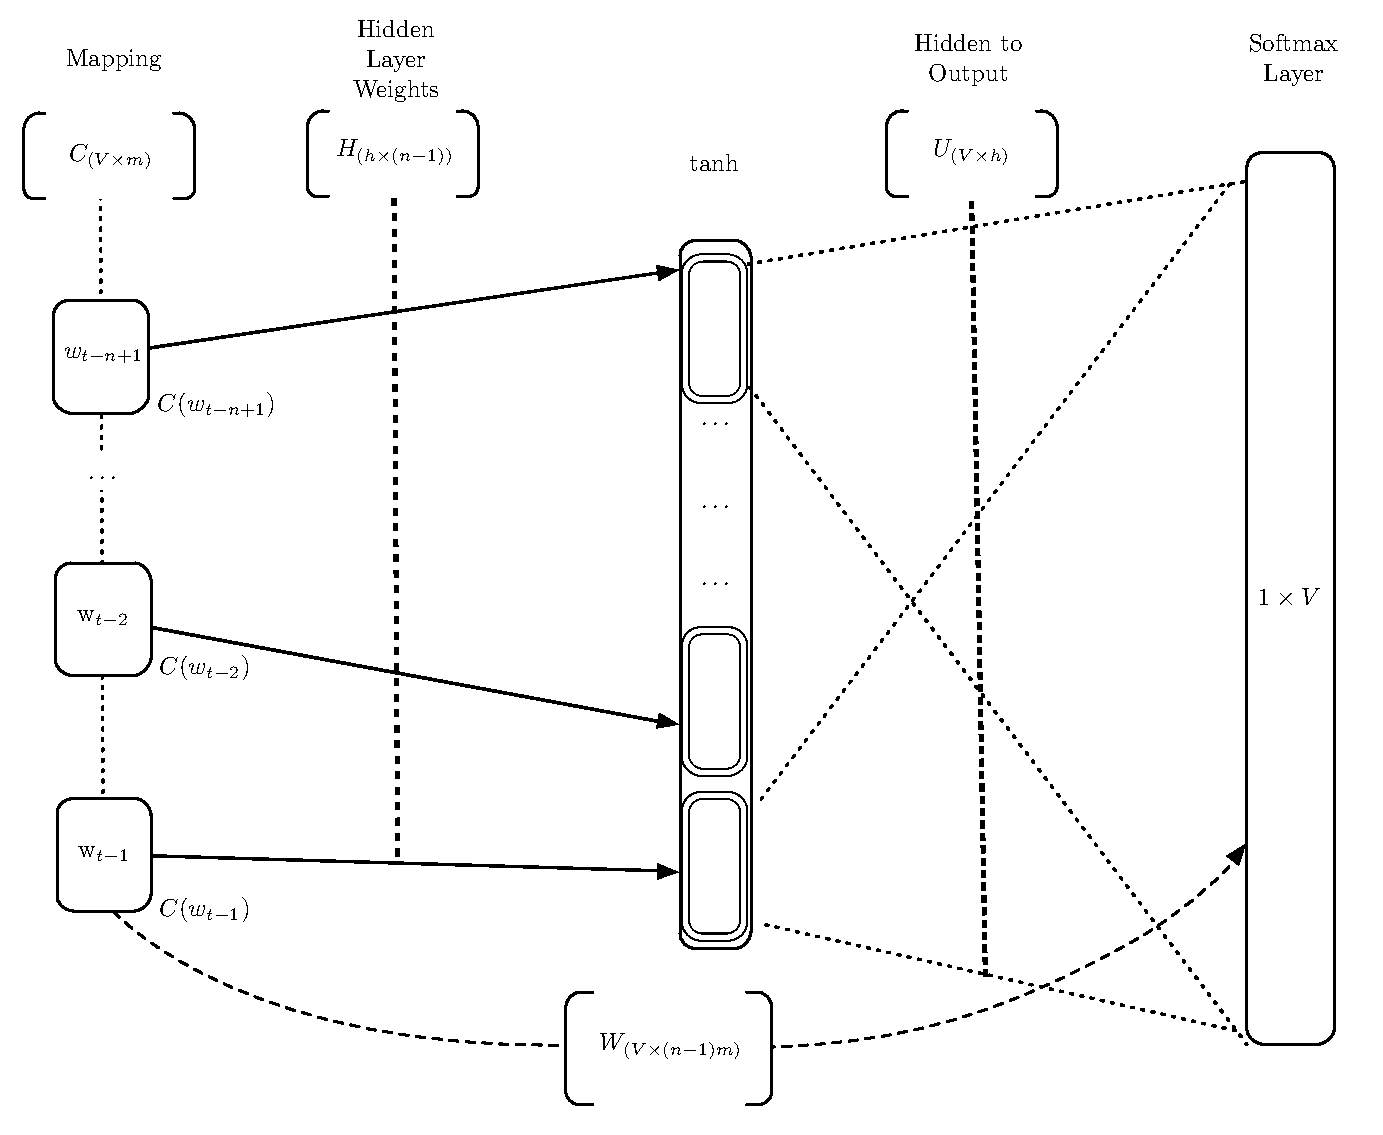
\includegraphics[width=0.8\textwidth]{images/bengio-nnlm.pdf}
    \caption{Feed Forward Neural Network Model Language Model Architecture.
       $C(i)$ is the $i$-th word feature vector.  \cite{Bengio:2003:NPL:944919.944966}.}
    \label{fig:NNLM_architecture}
\end{figure}

The neural network is trained using a gradient-based optimization algorithm
to maximize the training set \textit{log-likelihood}
\begin{equation}
 L(\theta) = \sum_t \log P(w_t | w_{t-n+1}, \ldots w_{t-1}) .
\end{equation}
The gradient $\frac{\partial L(\theta)}{\partial \theta}$
can be computed using the backpropagation algorithm \cite{Bishop:1995:NNP:525960}, extended
to provide the gradient with respect to $C$ as well as with
respect to the other parameters. 



The gradient   $\frac{\partial L(\theta)}{\partial
  \theta}$   is given by  :



\begin{equation*}
  \label{eq:nnlm-grad}
  \frac{\partial }{\partial \theta}\text{log}p_{\theta}^{n}(w_t=k) =
  \frac{\partial }{\partial \theta} e^{a_k} -  \frac{\partial }{\partial
    \theta}\text{log} \left( \sum_{l=1}^N e^{a_l} \right)
 \end{equation*}

\begin{equation}
\label{eq:dlogp-gradient}
  \frac{\partial }{\partial \theta}\text{log}p_{\theta}^{n}(w_t=k)  =  \frac{\partial }{\partial \theta} e^{a_k}  -   \frac{\partial }{\partial
    \theta}  \sum_{l=1}^N  p(w_t = l)  \frac{\partial }{\partial
    \theta}  e^{a_l}   
\end{equation}


As can bee seen from equation (\ref{eq:dlogp-gradient}), the  $\frac{\partial L(\theta)}{\partial
  \theta}$ is  expensive to calculate because implies a sum over all the scores $e^{a_{k}}$ over all possible words on the vocabulary.


\subsubsection{Model Complexity}
\label{sec:sub:sub:bengio_nnlm_complexity}

Figure \ref{fig:NNLM_architecture} is a graphical description of  the model.
It consists of three layers, input, projection and output layers. The N
previous word are encoded using 1-of-$V$ encoding, where $V$ is the size
of the vocabulary. $N$ previous word representation are concatenated using a
shared projection matrix to the projection layer $P$ (dimensionality $N
\times D$).  This layer is then conected to a hidden layer which is in turn
used to compute the probability distribution over all the words in the
vocabulary resulting in an output layer with dimensionality $V$. Therefore,
the computational complexity of each training example is:

\begin{center}
\begin{equation} Q = N \times D + N \times D \times H + H \times V,   \end{equation}
\end{center}

With the dominant term is $H \times V$, because of the gradient calculation
described above.
\cite{DBLP:journals/corr/abs-1301-3781}. Many solutions are proposed to avoid
the complexity in the last layer. One alternative is to use  hierarchical
versions of the softmax \cite{Morin05hierarchicalprobabilistic,6163930}.
The other alternative is to avoid is to avoid  normalized models by finding
a approximation to find the likelihood gradient \cite{NIPS2013_5165} . If binary tree representations are
used, the number of output units can decrease down to $log_2(V)$. Most
of the complexity will be then caused by  $N \times D \times H$.

% Of input, projection, hidden and output layers. At the input layer, N previous words are encoded
% using 1-of-V coding, where V is size of the vocabulary. The input layer is then projected to a
% projection layer P that has dimensionality N  D, using a shared projection matrix. As only N
% inputs are active at any given time, composition of the projection layer is a relatively cheap operation.


% Note that the gradient on most of $C$
% is zero (and need not be computed or used) for most of the columns of $C\ :$
% only those corresponding to words in the input subsequence have a non-zero gradient.
% Because of the large number of examples (millions to hundreds of millions),
% the only known practical [[optimization algorithm]] for  
% artificial neural networks 
% are online algorithms, such as [[stochastic gradient descent]]: the
% gradient on the log-likelihood of a single example at a time (one word in its
% context) or a mini-batch of examples (e.g., 100 words) is iteratively used to perform
% each update of the parameters.

% In a similar spirit, other variants of the above equations have been proposed (Bengio et al 2001, 2003;Schwenk and Gauvain 2004;Blitzer et al 2005; Morin and Bengio 2005; Bengio and Senecal 2008).

% The different  existing architecture will be described on section BLAH of
% this document.

\subsection{Recurrent Neural Net Language Model}

One of the major issues of the \ac{FNNLM}  approach is that
it has to used a fixed context that need to be specified at training time.
Therefore, the neural network only can see a limited number of preceding words when
predicting the next one.  A language model based on recurrent neural networks  do not use a context
with a size limit.  By using recurrent connection the information cycle
inside the networks for arbitraily long time. the \ac{RNNLM} proposed by
Mikolov use the so-called simple
recurrent neural network model. The network has an input layer $x$, hidden
layer $s$ (also called context layer or state) and output layer $y$. Input to
the network in time $t$ is $x(t)$, output is denoted as $y(t)$, and $s(t)$ is
state of the network (hidden layer). Input vector $x(t)$ is formed by
concatenating vector $w$ representing current word, and output from neurons in
context layer $s$ at time $t - 1$. Input, hidden and output layers are then
computed as follows \cite{conf/interspeech/MikolovKBCK10}:.

\begin{equation} x(t) = (w(t), s(t-1))  \end{equation} 

\begin{equation} s_j(t) = f \left( \sum_{i}{x_i(t)u_{ij}}
  \right)   \end{equation}

\begin{equation}  y_v(t) = g \left( \sum_{j}{s_j(t)h_{kj}}
  \right)   \end{equation}


Where   $f(z)$ is \textit{sigmoid} activation function and $g(z)$  is the
traditional   \textit{softmax}.  $y_v(t)$ represents the probability of that
the next word is $W_v$.

Figure \ref{fig:RNNLM_architecture} despicts the architecture of the simple
recurrent neural network this model is based on. Similar to the \ac{FNNLM},    $w(t)$ represents the word in time $t$ encoded using 1-of-$V$ coding.  $s(t-1)$ represents the output values in the
hidden layer from the previous time step. Therefore $x(t)$, the input, has
the size of the vocabulary $V$ and of vector $s(t-1)$. After the network is
trained, the output represent the probability represented by equation (\ref{eq:lm_probability}).  \cite{mikolovphd2012}.

\begin{figure}[hptb!]
    \centering
    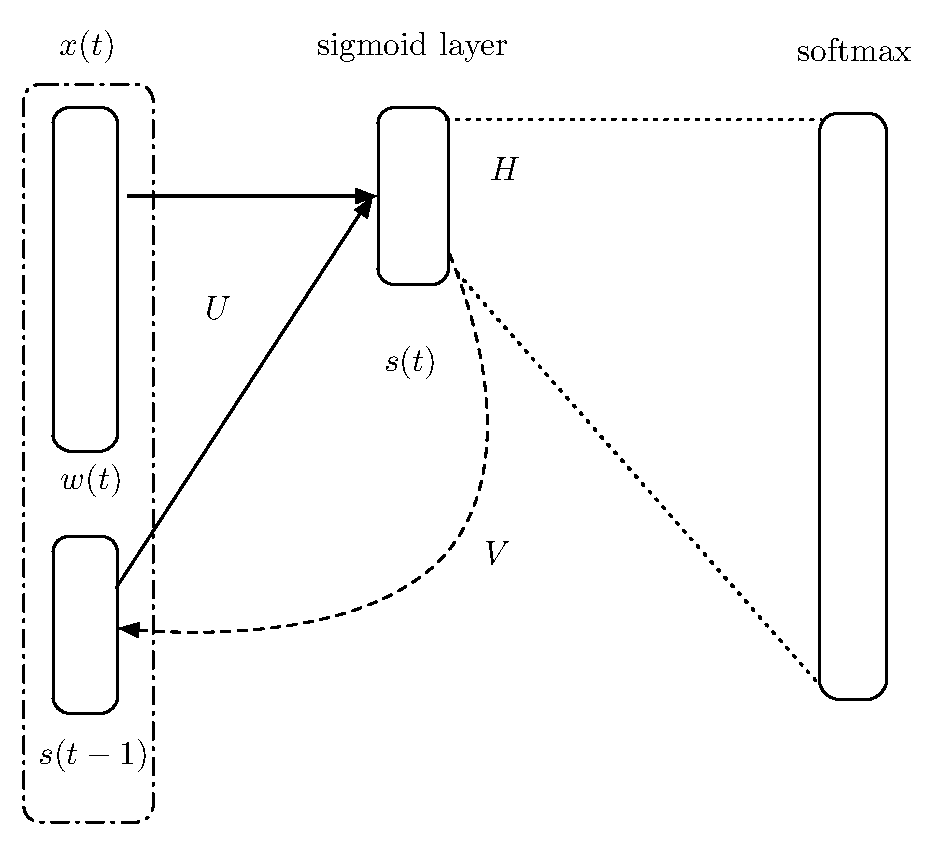
\includegraphics[width=0.6\textwidth]{images/mikolov-rnnlm.pdf} 
    \caption{Recurrent Neural Network Language Model Architecture}
    \label{fig:RNNLM_architecture}
\end{figure}

The network is trained by  stochastic gradient descent using the
\textit{backpropagation} algorithm \cite{Bishop:1995:NNP:525960}.


\subsubsection{Model Complexity}
\label{sec:sub:sub:mikolov_rnnlm_complexity}

Assuming that the hidden layer and the word representation share the same
dimensionality with the hidden layer, the complexity per training example of the RNN model is
given by:


\begin{equation} Q = H \times H + H \times V,   \end{equation}

In a similar fashion to the \ac{FNNLM}, the term $H \times V$ can be
efficiently reduced to $H \times log_2(V)$ by using the hierarchical softmax
formulation. Thus, most of the complexity comes $H \times H$.

% Recurrent neural networks do not use limited size of con- text. By using recurrent connections, information can cycle in
% side these networks for arbitrarily long time (see [5]). However, it is also often claimed that learning long-term dependencies by stochastic gradient descent can be quite difficult [6].
% In our work, we have used an architecture that is usually called a simple recurrent neural network or Elman network [7]. This is probably the simplest possible version of recurrent neu- ral network, and very easy to implement and train. The network has an input layer x, hidden layer s (also called context layer or state) and output layer y. Input to the network in time t is x(t), output is denoted as y(t), and s(t) is state of the network (hidden layer). :




% A major deficiency of Bengio’s approach is that a feedfor- ward network has to use fixed length context that needs to be specified ad hoc before training. Usually this means that neural networks see only five to ten preceding words when predicting the next one. It is well known that humans can exploit longer context with great success. Also, cache models provide comple- mentary information to neural network models, so it is natural to think about a model that would encode temporal information implicitly for contexts with arbitrary lengths.


\subsection{Mikolov's Neural Network Language Model}
\label{sec:mikolov-neural-net-model}



Mikolov neural network language model uses additional approach to the one
described back in section \ref{subsec:fwd-neural-net-lm}.  The neural network
architecture is split in two steps. In the first one the architecture trains
a bigram neural network. Given a word $w$ from a vocabulary $V$, the neural
network tries to estimate the the probability distribution of the next word
in the text. Both the input and output are of size $|V|$, were the words a
usually is encoded with 1-of-$K$ encoding, with $K=|V|$.  Theres is one hidden layer of
size $|D|$ has an arbitrary size (reported by the authors  to range from 20-60). As with the
other models, the output layer  is a  softmax layer. The nework is trained
using the standard \textit{backpropagation} algorithm
\cite{conf/icassp/MikolovKBGC09}. 




The second step consists of  A $N$-gram network. The network is trained in a
similar waym, however the input vector does not encode previous word in
history using 1-of-$K$ encoding, but is formed using $N-1$ projections from
the  bigram network. These projections are the learned weights of dimension
$|D|$ learned by the big-gram network. Figure \ref{fig:mikolov_nnlm_architecture} show a schematic of the
two-network architecture 





\subsubsection{Model Complexity}

As this model is formed by two parts, the model complexity depends wheter the
full model is desired to be estimated or not. If one is only interested in
the word representations, i.e. the projections from the big-gram network the
complexity is reduced  by the simplicity of the model, regardless of the
quality of the representation obtained.  As reference the full model
complexity is described: 


\begin{equation} Q_1 = V \times D + D \times V  \end{equation}

\begin{equation} Q_2 =  N \times D \times H + H \times V   \end{equation}

\begin{equation} Q = Q_1 + Q_2
\end{equation}

With $Q_1$ and $Q_2$ the complexity of the bigram network and the $N$-gram
network respectively. Although not mentioned by the authors, efficiency
improvement can be achieved by using hierarchical formulations of the softmax
can be used. If it is used, most of the complexity  lies in the  $N \times D \times
H$ term of $Q_2$.

\begin{figure}[hptb!]
    \centering
    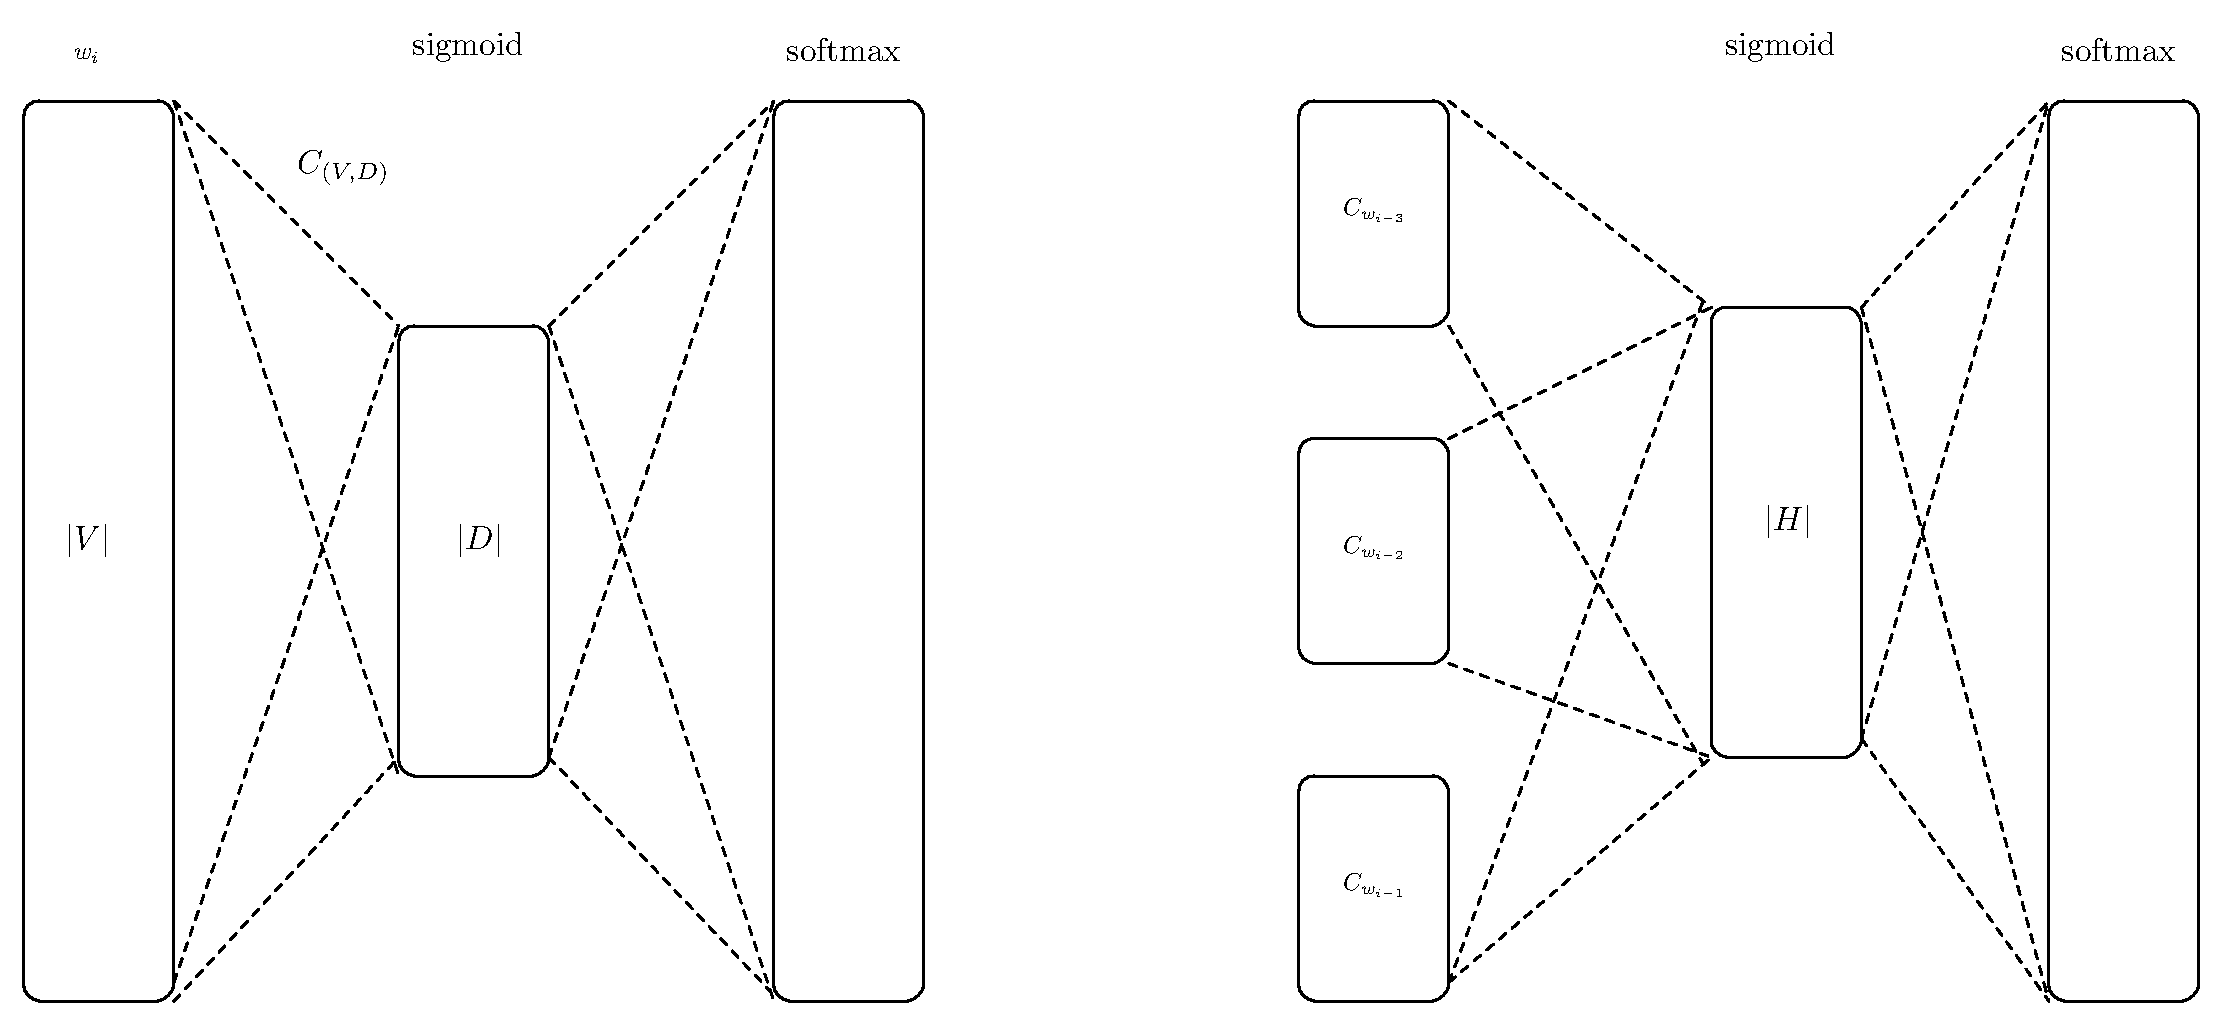
\includegraphics[width=1.0\textwidth]{images/mikolov-fnnl-latex.pdf} 
    \caption{Mikolov's Neural Network Language Model Architecture}
    \label{fig:mikolov_nnlm_architecture}
\end{figure}
  

% \subsection{Mikolov Neural Network Model}



\section{Deep Learning}
\label{sec:deep_learning}


\section{Represenation of Text}
\label{sec:rel_represenation_text}


\subsection{Local Representations}
\label{sec:rel_local_representation}

\subsubsection{N-grams}
\label{sec:sub_ngrams}

\subsubsection{Bag-of-words}
\label{sec:rel_bow}

\subsubsection{1-of-N coding}
\label{sec:1_of_coding}

\subsection{Continuous Representations}
\label{sec:sub_continuous_representation}

\subsubsection{Latent Semantic Analysis}
\label{sec:rel_local_representation}

\subsubsection{Latent Dirichlet Allocation}
\label{sec:rel_lda}

\subsubsection{Distributed Representations}
\label{sec:dis_rep}





%%% Local Variables: 
%%% mode: latex
%%% TeX-master: "../main.tex"
%%% End: